% !TeX encoding = utf8
% !TeX spellcheck = fr

\chapter{Calculateur de vol}\label{cha:glide}
Ce chapitre explique comment le calculateur de vol d'\xc{} fonctionne.
Il est recommandé de le lire afin de connaître les détails spécifiques aux calculs de navigation et de savoir se servir correctement du logiciel.
Des connaissances basiques du vol sur la campagne sont présupposées.
Les pilotes de compétition ainsi que les vélivoles faisant des vols de loisirs sur la campagne ont aussi intérêt à le lire~!


\section{Les modes de vol}\label{sec:flightmodes} 

Afin de réduire le charge du travail du pilote, \xc{} accomplit différents calculs selon la phase actuelle du vol.
\xc{} peut les faire sans interaction avec le pilote au cours du vol.
Les différences entre modes se retrouvent en particulier dans les différents affichages, calculs, et informations de vol.
Les quatre modes utilisés par \xc{} sont~:
\begin{itemize}
\item Transition
\item Spirale
\item Arrivée
\item Abandon
\end{itemize}
\xc{} détecte automatiquement le passage entre les modes ``Spirale'' et ``Transition''.
Le mode Spirale est activé quand le planeur tourne (typiquement après trois quart de tour).
Après environ 30~secondes de vol en ligne droite, le logiciel passera du mode Spirale au mode ``Transition''.
Ainsi, le passage est basé sur une règle très simple.

Il est aussi possible de basculer en mode Spirale sur la base d'une action externe (par exemple, à partir d'un interrupteur activé par le pilote).

Le mode Arrivée s'active quand le planeur est au-dessus du plan d'arrivée par rapport au circuit et aux marges de sécurité paramétrés.
L'altitude requise dépend en premier lieu du calage MacCready sélectionné, mais aussi de la hauteur au-dessus du sol.
Si vous enroulez une ascendance pour augmenter les marges de sécurité alors qu'\xc{} est en mode Arrivée, le logiciel passera en mode Spirale.
Puis, une fois l'ascendance quitté et les conditions d'arrivée réunies (c.-à-d.\ au-dessus du plan d'arrivée en considérant le calage MacCready et le relief), le logiciel reviendra en mode Arrivée.

À titre d'exemple, une fonction puissante liés aux modes de vol est le basculement entre des stratégies différentes de calage MacCready.
Si vous décidez de laisser \xc{} gérer automatiquement le calage, il prendra une valeur basée sur les ascendances passées qui ont fonctionnées, et ce jusqu'à l'arrivée.
Pour l'arrivée, le MacCready instantané est fait pour obtenir une durée de parcours minimale ou une autre condition que vous avez paramétré pour l'arrivée (voir section~\ref{sec:auto-maccready}).
\config{final-glide} Ainsi, le passage en mode Arrivée est basé sur une série de conditions tactiques calculée de manière sophistiquée.

Vous pouvez forcer \xc{} à passer en mode Arrivée en sautant les points de virage restants, si, par exemple, les conditions de vol se dégradent et que vous décider de rentrer.

Le mode Abandon est déclenché manuellement afin de vous donner un contrôle total en cas d'urgence par un menu.
Ce n'est pas automatique --- c'est à vous de décider.
Techniquement, le mode Abandon peut être vu comme un cas particulier du mode Arrivée qui gèrent simultanément plusieurs possibilités d'atterrissage.
Toutefois, en pratique, le mode Abandon vous aide simplement dans votre choix urgent de décider d'où et de comment atterrir (voir~\ref{sec:taskabort}).
Dans ce cas, un calage MacCready de sécurité est défini.
\config{safetyMC} Ainsi, la sélection du mode Abandon est basé uniquement sur la décision du pilote.

Parce que les différents modes de vol se différencient par les informations affichées, l'utilisateur fréquent d'\xc{} peut s'habituer à voir différents type d'affichage.
Ceci est la perception par défaut lorsque l'on a installé \xc{} sans avoir fait de fortes modifications à la configuration.
Comme presque toujours avec \xc, le comportement de l'affichage peut être modifié, apportant une plus-value à l'utilisateur avancé.
Mais modifier des choses dans \xc{} ne change pas les conditions de passage entre les différents modes.

Afin de bénéficier au maximum du concept de mode de vol, \xc{} affichera \emph{toujours} le mode actif.
Un petit symbole est affiché dans le coin inférieur droit de la carte, indiquant le mode de vol actuel du calculateur~:

\begin{tabular}{c c c c}%{c c c c}

\includegraphics[angle=0,width=0.75cm,keepaspectratio='true']{icons/mode_cruise.pdf} &

\includegraphics[angle=0,width=0.75cm,keepaspectratio='true']{icons/mode_climb.pdf} &

\includegraphics[angle=0,width=0.75cm,keepaspectratio='true']{icons/mode_finalglide.pdf} &

\includegraphics[angle=0,width=0.75cm,keepaspectratio='true']{icons/mode_abort.pdf}\\
(a) & (b) & (c) & (d)
\end{tabular}

\begin{description}
\item[Transition (a)] Le planeur ne spirale pas, et soit il n'y a pas de circuit actuellement activé, soit le prochain point de virage n'est pas le dernier.
\item[Spirale (b)] Le planeur est en spirale (même s'il ne monte pas).
\item[Arrivée (c)] Le planeur ne spirale pas et le point de virage actif est le dernier du circuit.
\item[Abandon (d)] Ce mode activé manuellement affiche les différents terrains/champs ``posables'' (voir section~\ref{sec:taskabort})
\end{description}

Le concept de différents modes de vol permet encore plus d'automatisation~:
\begin{itemize}
\item \config{screenpages} Les InfoBoxes peuvent être configurées différemment pour chaque mode de vol (voir section~\ref{sec:infoboxandpages})
\item \config{circlingzoom} Le niveau de zoom peut être différent entre le mode Spirale et les autres modes (c'est le `zoom Spirale', voir Section~\ref{sec:zooming}).
\item \config{variogauge} Basculer l'affichage de l'échelle du vario entre Vario (taux de montée réel) en mode Spirale et Netto (taux de montée de la masse d'air autour de vous) en mode Transition (voir section~\ref{sec:variometer}).
\item \config{thermalassistant} En mode Spirale, afficher l'``assistant thermique'', un petit diagramme polaire représentant l'ascendance sur la trajectoire circulaire (voir section~\ref{sec:thermal-assistant}).
\item \config{traildrift} Afficher le mode dit ``dérive compensée'', dessinant une trace compensée du vent pour les cercles que vous parcourez, représentant mieux le cisaillement du vent (voir section~\ref{sec:trail}).\end{itemize}

Notez que cette liste donne juste quelques exemples parmi tous les éléments modifiables.
Vous découvrerez les nombreuses autres possibilités offertes par les modes de vol en poursuivant la lecture de ce manuel.
Soyez-y attentif car le concept de modes de vol est un élément fondamental d'\xc.
Un autre élément fondamental est la façon structurée d'afficher l'information.
Des détails supplémentaires sont fournis dans la section~\ref{sec:infoboxandpages} ``InfoBoxes et pages d'écran''.\config{screenpages}


\section{Calage MacCready}

Le calage MacCready peut être ajusté de plusieurs façons~:
\begin{itemize}
\item Pour les écrans tactiles/les souris, sélectionnez l'InfoBoxe MacCready, puis utilisez les touches Haut/Bas.
\item Quand un variomètre intelligent (supporté) est connecté, l'ajustement du calage MacCready sur le variomètre modifiera le calage MacCready d'\xc, conformément aux réglages de synchronisation du périphérique (voir section~\ref{conf:comdevices}).
\end{itemize}
De plus, un mode MacCready automatique est disponible, comme décrit en section~\ref{sec:auto-maccready}.


\section{Polaire}\label{sec:glidepolar}

La définition des polaires de nombreux planeurs de différentes classes est intégrée dans \xc.
\menulabelr{\bmenug{Config 2/3}\blink\bmenug{Planeur}}
Si votre planeur n'est pas dans la liste, le choix d'un planeur aux performances voisines mais pas supérieures peut servir de réglage approximatif. \config{polar}
Bien entendu, pour des calculs précis, il faut utiliser la polaire correspondant à votre planeur.
Il ne suffit pas de définir la bonne polaire~: pour des calculs précis, la masse totale du planeur en vol doit être définie dans \xc.
La check-list avant vol de votre \xc{} contient vraisemblablement une vérification du bon paramétrage des ballasts, en particulier de la masse à vide.
Parce qu'\xc{} n'a pas de paramètre ``poids du pilote'', vous pouvez l'inclure soit dans la masse totale à vide, soit le paramétrage des ballasts.

En plus de la configuration de la polaire et des ballasts, le polaire est modifiable en vol afin de tenir de la dégradation des performances par les moucherons et par la pluie.

L'accumulation de moucherons sur le bord d'attaque, ainsi que la pluie sur les ailes, affectent les performances aérodynamiques.
C'est au pilote d'évaluer la dégradation des performances aérodynamiques et de modifier la valeur des moucherons.
La valeur de la dégradation estimée est représentée par un pourcentage de dégradation par rapport à la polaire parfaite.
Par exemple, avec les moucherons à 0~\%, le planeur est supposé se comporter comme un planeur propre.
Avec les moucherons à 50~\%, le taux de chute du planeur est multiplié par deux par rapport au planeur propre.
Les calculs de dégradation sont linéaires.

\menulabel{\bmenug{Info 1}\blink\bmenug{Analyse}}
\begin{center}
\includegraphics[angle=0,width=\linewidth,keepaspectratio='true']{figures/cut-clean-dirty-polar.png}
\end{center}
Sachant cela, un réglage pertinent pour une aile extrêmement contaminée par des moucherons pourrait aller jusqu'à 30~\%.
Seuls des tests permettront de connaître les valeurs correctes pour les moucherons, car la dégradation des performances diffèrent d'un planeur à l'autre.

Une autre façon de faire est d'activer la fonction ``Moucherons automatique'' qui ajoute 1~\% de moucherons après chaque heure de vol.
Cette fonction est accessible par 

\button{Config 1}\blink\button{Système}\blink\button{Calculateur}
\blink\\\button{Paramètres de sécurité}\blink\button{Moucherons auto.}

Le paramètre ``Ballast'' est en litres.
La masse à vide rentrée pour le planeur peut permettre la prise en compte les poids de différents pilotes.
En vol à vide, un pilote lourd pourrait peut-être mettre la valeur de ``Ballast'' à 15~litres pour que la polaire soit correctement ajustée par rapport à l'accroissement de la masse dans le cockpit.

\begin{center}
\menulabel{\bmenug{Info 1}\blink\bmenug{Analyse}}
\includegraphics[angle=0,width=\linewidth,keepaspectratio='true']{figures/overlay-non-balasted-polar.png}
\end{center}


\section{Paramètres de vol}\label{sec:flight-setup}
La fenêtre des paramètres de vol permet de modifier la masse totale du planeur à la fois avant et pendant le vol, ainsi que de régler la pression QNH.\@

\menulabel{\bmenug{Config 1}\blink\bmenug{Vol}}
\begin{center}
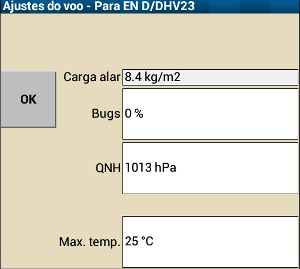
\includegraphics[angle=0,width=0.45\linewidth,keepaspectratio='true']{figures/dialog-basicsettings.png}
\end{center}

Le paramètre ``Moucherons'' défini la dégradation de la performance aérodynamique de l'aile causée par la contamination au cours d'un long vol.
Avec un ``moucherons'' mis à 0~\%, \xc{} utilisera une polaire propre.
Avec un ``moucherons'' mis à 50~\%, la polaire sera dégradée et doublera le taux de chute à une vitesse donnée.

Le paramètre ``ballast'' est utilisé pour modifier la polaire afin de rendre compte de l'eau présente dans les ballasts pendant le vol.
Les ballasts sont affichés en litres et doivent correspondre à la valeur d'eau ajoutée dans les ballasts avant le vol.
Le paramétrage des ballasts modifie la polaire pour prendre en compte la masse fournie pour les ballasts.

Utilisez cette fenêtre à la fois avant et pendant le vol pour paramétrer le pression moyenne au niveau de la mer, aussi appelée pression QNH.\@
\xc{} utilise cette valeur pour convertir les niveaux de vol en altitudes.
Si le logiciel est connecté à un variomètre intelligent muni d'un capteur de pression, l'altitude est mise à jour dans cette fenêtre lors de l'ajustement de le pression QNH.\@
Cela permet aussi de caler facilement la pression QNH au sol sur la base de l'altitude du terrain.

La température maximale prévue au sol est utilisée par l'algorithme de prévision de la convection (voir section~\ref{sec:convection-forecast}) pour la détermination de la hauteur estimée du plafond de la convection et de la base des nuages.

\tip{} Il est possible de configurer \xc{} pour afficher la fenêtre des paramètres de base au démarrage.

Au démarrage, une fois que le GPS a acquis une position, et si un appareil délivrant la pression atmosphérique est connecté (ex~: Vega, AltairPro, FLARM), la mise à jour du QNH est automatique.
Ce réglage du QNH fait en sorte que l'altitude barométrique corresponde à celle du terrain.

Le QNH est mis à jour uniquement si l'appareil est au sol depuis plus de 10 secondes, afin que si \xc{} est redémarré en vol, le QNH ne soit pas remis à jour.
La mise à jour automatique n'est possible que si l'appareil se situe sur un terrain de la base de données.

\section{Affichage vitesse à suivre}

Quand le calculateur est connecté à un variomètre intelligent délivrant la mesure de la vitesse indiquée, un indicateur de vitesse à suivre est affiché sur la droite de la carte sous la forme de chevrons.
Si la vitesse du planeur est inférieure à la vitesse à suivre, des chevrons rouges pointant vers le bas sont affichés.
Si le planeur vole plus vite que la vitesse à suivre, ce sont des chevrons verts pointant vers le haut.
Si la vitesse du planeur est proche de la vitesse à suivre, il n'y a pas de chevrons.

En fonction de la configuration, les chevrons de vitesse à suivre s'affichent sur la droite de la carte ou dans le cadran du vario.


\section{Vitesse de vol}\label{sec:stf}

\xc{} calcule en permanence 2~vitesses de vol~:
\begin{description}
\item[Vitesse MacCready] La meilleure vitesse de vol en transition et en air calme.
Le vent est pris en compte si l'on est en mode ``Arrivée''.
\item[Vitesse de vol en dauphin] C'est la meilleure vitesse instantanée en vol en air ascendant ou descendant.
Le vent est pris en compte si l'on est en mode ``Arrivée''.
\end{description}

Le pilote peut configurer une vitesse de manœuvre maximale afin de limiter à des valeurs réalistes la vitesse de vol calculée avec le MacCready.

Les pilotes peuvent avoir leurs préférences lors des transitions entre ascendances~: le vol MacCready à vitesse constante entre 2~ascendances, ou le vol en `dauphin' qui demande de voler à des vitesses variables selon une valeur de vitesse de vol en dauphin changeant continuellement.

%\begin{maxipage}
\begin{center}
\includegraphics[angle=0,width=1.0\linewidth,keepaspectratio='true']{figures/figure_speed_to_fly-fr.pdf}
\end{center}
%\end{maxipage}

Un paramètre de configuration `Vitesse de croisière bloquée' (voir section~\ref{sec:final-glide}) peut être utilisé pour définir si c'est la vitesse de vol en dauphin ou la vitesse constante qui est utilisée.
L'InfoBoxe `V Opt' montre la vitesse optimale selon le type de calcul qui est sélectionné.
Connecté à un variomètre intelligent Vega, les sons de la ``vitesse à suivre'' reflètent cette vitesse optimale.


\section{Vitesse de vol et risque}\label{sec:safety-factor}

Le calcul de vitesse de vol peut être compensé en fonction du risque (risque~= vache~= altitude), dans lequel le calage MacCready utilisé pour calculer la vitesse de vol (à la fois en mode ``vitesse constante'' et en mode ``vitesse en dauphin'') est réduit quand le planeur se rapproche du sol.

De nombreux pilotes diminuent le calage du MacCready quand ils perdent de l'altitude et se rapprochent du sol --- cette fonctionnalité le fait automatiquement.
Les méthodes de calcul de \xc{} sont inspirées de la publication de John Cochrane, ``MacCready Theory with Uncertain Lift and Limited Altitude'', \emph{Technical Soaring}, 23 (3) (juillet 1999) 88--96.

\url{faculty.chicagobooth.edu/john.cochrane/soaring/docs/newmcred.pdf}

Un paramètre de configuration $\gamma$ (`Coef.\ risque sur calage', dans le menu Config, sous la page `Paramètres de sécurité') contrôle comment le ``risque MacCready'' est calculé.
Le facteur $\gamma$ détermine une fonction faisant varier le calage MacCready utilisé pour les calculs de la vitesse optimale.
Il prend en considération~:
\begin{itemize}
\item $h_{top}$, la hauteur de la masse d'air convective ``utilisable'' par le pilote.
Celle-ci est définie par la hauteur maxi.\ au-dessus du sol atteinte en ascendance (généralement proche de la base des nuages)~;
\item $h$, la hauteur au-dessus du sol à laquelle le pilote souhaite abandonner le circuit, c.-à-d.\ se mettre en prise de terrain pour se vacher ou se diriger vers un point de virage posable.
\end{itemize}
Le paramètre $\gamma$ représente en fait la fraction $h/h_{top}$, Une valeur faible de $\gamma$ traduit l'acceptation d'un risque plus important qu'une valeur importante de $\gamma$.

Si $\gamma$ est laissé à la valeur par défaut (0.0), il n'y pas de diminution du calage MacCready lorsque le sol se rapproche --- le risque MacCready est alors le même que le MacCready paramétré.
Pour un $\gamma$ réglé à 1.0, le risque du MacCready évolue linéairement avec le rapport $h/h_{top}$.
Pour des valeurs intermédiaires de $\gamma$, le risque MacCready varie graduellement avec le rapport $h/h_{top}$ de façon à ce que le risque MacCready soit faible uniquement lorsque l'on vole bas.

Des valeurs faibles de $\gamma$ sont préférables pour les pilotes ne souhaitant pas ralentir quand ils se rapprochent du sol.
Ils assument alors un fort risque de vache et recherchent une vitesse maximale.
Des valeurs élevées de $\gamma$ doivent être utilisées par les pilotes prudents qui veulent diminuer le risque de vache et ne recherchent pas la vitesse moyenne maximale.

Une valeur de $\gamma$~=~0.3 est un bon compromis.

\begin{center}
\includegraphics[angle=0,width=0.9\linewidth,keepaspectratio='true']{figures/riskmc.png}
\end{center}


\section{Hauteurs de sécurité}\label{sec:safety-heights}

Trois hauteurs de sécurité existent dans \xc{} afin de pouvoir définir des marges de sécurité par rapport au sol dans les calculs.

Ces hauteurs de sécurité sont~:
\begin{description}
\item[Hauteur d'arrivée (a)] Hauteur minimale au-dessus du sol à laquelle le planeur doit arriver.
Généralement, vous voulez y inclure la hauteur pour un tour de piste en sécurité, ainsi qu'une marge de sécurité par rapport aux possibles mouvements verticaux et horizontaux de la masse d'air, et les erreurs de calcul de vitesse et de cap.
Cette valeur est utilisée dans les calculs d'arrivée ainsi que dans la recherche et l'affichage des terrains atteignables (c.-à-d.\ ceux qui sont en local).
\item[Garde au sol (b)] Hauteur minimale au-dessus du sol qu'une route calculée doit respecter pour être valide.
La garde au sol impacte le calcul de la ``zone atteignable en plané''.
Si le long de la trajectoire d'arrivée prévue la garde au sol n'est pas respectée, une épaisse croix rouge apparaît à l'endroit de la violation de la garde au sol.
Si la carte des reliefs n'est pas valable ou hors de portée, le calcul de ``zone atteignable en plané'' et l'affichage de la croix sont désactivés.
\item[Hauteur de dégagement] Hauteur sol en dessous de laquelle il est recommandé aux pilotes de considérer l'abandon du circuit et de se concentrer sur la recherche d'un terrain posable.
À ce jour, cette hauteur de dégagement n'impacte en aucune façon les calculs de \xc, mais il en est fait référence dans le manuel d'utilisation.
\end{description}

%\begin{maxipage}
\begin{center}
\includegraphics[angle=0,width=\linewidth,keepaspectratio='true']{figures/figure_terrain-fr.pdf}
\end{center}
%\end{maxipage}

\warning{}
Ces hauteurs de sécurité peuvent être mises à zéro, mais ceci est fortement déconseillé car tous les calculateurs de vol, instruments et sources de données (carte du relief par exemple) sont sujets à des erreurs et/ou imprécisions.
De plus la masse d'air dans laquelle le planeur évolue est instable et soumise à des évolutions imprévisibles.

\xc{} évalue l'altitude au-dessus du niveau de la mer (ASL) de chaque point de virage ou terrain posable soit à partir du fichier de points de virage ou, si aucune altitude n'est définie dans le fichier de points de virage, à partir de la carte de relief.

\textbf{L'altitude d'arrivée estimée qui est affichée à côté du point de virage posable est calculée par défaut à partir de la meilleure finesse calculée avec un calage MacCready nul (MC$=0$) et en tenant compte du vent.
Cependant, un calage MacCready de sécurité à utiliser pour ce calcul est paramétrable, comme décrit ci-dessous.}

Les aérodromes et champs vachables sont affichés comme atteignables (``en local'') si la hauteur d'arrivée estimée par rapport au sol est supérieure à la hauteur d'arrivée paramétrée, et si la trajectoire calculée ne rencontre pas le relief (en tenant compte de la garde au sol).

Dans tout les cas, si le signal de collision apparaît (croix rouge), alors le planeur doit reprendre de l'altitude afin d'arriver à destination en sécurité.

Lors du calcul de la hauteur estimée d'arrivée sur les points posables (pour affichage sur la carte et en mode ``Abandon''), une valeur de sécurité de calage du MacCready est paramétrable dans le menu Config.
La valeur par défaut est zéro.
Des valeurs plus élevées de ce paramètre rendent le calcul de hauteur d'arrivée plus pessimiste, donc minimisant les risques.


\section{Le calculateur d'arrivée}

Le calculateur d'arrivée utilise de nombreuses sources de données pour déterminer l'altitude nécessaire pour atteindre votre objectif ou le prochain point de virage.
Ce sont~:

\begin{itemize}
\item La polaire du planeur~;
\item La vitesse et la direction du vent~;
\item La distance et le cap pour atteindre l'objectif ou le point de virage~;
\item Le calage MacCready~;
\item L'altitude de l'objectif ou du point de virage~;
\item Une hauteur de sécurité spécifiée par l'utilisateur (hauteur d'arrivée et garde au sol)~;
\item L'énergie totale du planeur si \xc{} est connecté à un instrument lui donnant la vitesse air instantanée.
\end{itemize}

Des paramètres ci-dessus découlent deux altitudes~:
\begin{description}
\item[Altitude requise] Altitude nécessaire pour atteindre l'objectif.
Cette altitude comprend toute hauteur de sécurité paramétrée~;
\item[Hauteur différentielle] calculée à partir de l'altitude nécessaire pour atteindre l'objectif (incluant la hauteur de sécurité), plus l'altitude de la cible (ASL), moins l'altitude du planeur (ASL).
Cette hauteur représente soit la hauteur au-dessus (ou en dessous) du plan d'arrivée, soit la hauteur d'arrivée au-dessus (ou en dessous) de l'objectif.
Si aucune altitude n'est définie pour l'objectif (dans le fichier des points de virage), \xc{} utilise l'altitude de l'objectif sur la carte du relief.
\end{description}

La méthode de calcul du plan d'arrivée est étendue au calcul des `altitudes requises' et des `hauteurs différentielles' pour terminer le circuit.
On parle parfois de cette fonctionnalité comme étant le calcul permanent du plan d'arrivée.
La hauteur différentielle pour terminer le circuit est affichée en permanence sur la partie gauche de la carte et est représentée sous forme d'une flèche et de chiffres.

L'altitude requise est convertie en énergie potentielle, ceci afin de pouvoir prendre en compte l'énergie cinétique du planeur et la convertir en hauteur (énergie potentielle).
L'énergie cinétique qui est convertible en hauteur est calculée à partir de la différence entre la vitesse air instantanée et la vitesse air à finesse max.
Cette valeur sera nettement plus précise si \xc{} est connecté à un instrument lui donnant la vitesse air instantanée.
Sinon la vitesse air instantanée est estimée à partir de la vitesse estimée du vent et de la vitesse sol (GPS).


\section{Affichage de l'altitude différentielle requise}

Sur la partie gauche de la carte, une case affiche l'altitude différentielle nécessaire pour terminer le circuit, ou atteindre le point de virage final.
Si le planeur est au-dessus de l'altitude minimum requise, une flèche verte pointe vers le haut au-dessus de la case, indiquant la hauteur excédentaire.

Si le planeur est en dessous de l'altitude minimale requise, une flèche rouge pointe vers le bas est affichée, représentant le manque de hauteur pour atteindre l'objectif.
Si, cependant, il y a des terrains posables en ``local'' mais que le planeur n'a pas suffisamment de hauteur pour terminer le circuit, la flèche est de couleur ambre.

\begin{center}
\begin{tabular}{c c}
\emph{Au-dessus} & \emph{En-dessous} \\
\includegraphics[angle=0,keepaspectratio='true']{figures/cut-fg-above.png} &
\includegraphics[angle=0,keepaspectratio='true']{figures/cut-fg-below.png} \\
\multicolumn{2}{l}{La gamme de la flèche d'arrivée est $+/-$ 500~mètres.} \\
\multicolumn{2}{l}{Au-delà de cette gamme, un chevron est affichée au bout de la flèche.}
\end{tabular}
\end{center}
\tip{}
Notez bien que la hauteur indiquée sous le plan d'arrivée n'est pas une simple différence entre la plan d'arrivée et l'altitude actuelle.
Selon la configuration de `Inclure la dérive en spirale' (On), l'indicateur `En dessous' montre le gain de hauteur nécessaire en spirale. \config{predict-drift}
La hauteur nécessaire pourrait être significativement plus importante en cas de vent de face, mais aussi un peu moins forte avec du vent arrière.
Si `Inclure la dérive en spirale' est sur Off, c'est simplement la différence d'altitude brute.



\subsection*{Double flèche et altitude différentielle}

La flèche d'arrivée a été modifiée pour montrer l'effet du calage MacCready sur l'altitude différentielle nécessaire pour terminer le circuit.
L'affichage d'une flèche creuse montre \emph{l'altitude différentielle avec un calage MacCready à zéro}, tandis que la flèche pleine affiche l'altitude différentielle avec le calage MacCready présent.

Le nombre dans la boite à la base de la flèche montre toujours l'altitude différentielle calculée avec le calage MacCready présent.

Exemples d'affichages dans différentes situations avec la demi-flèche additionnelle \emph{MacCready~$=0$}~:

\begin{description}
\item[Au-dessus du plan] (MacCready présent~$=0,7$)
La flèche verte pleine montre qu'au calage MacCready présent, le planeur est au-dessus du plan d'arrivée (flêche pleine).
La demi-flèche montre la hauteur excédentaire.
\smallsketch{figures/fig-finalglide-allabove.png}

\item[En-dessus/au-dessous du plan d'arrivée] (par ex. MacCready~$=1,8$)
Ici on voit qu'avec le calage MacCready présent, le planeur est en dessous du plan d'arrivée (flèche pleine ambre).
La demi-flèche verte creuse montre qu'avec un calage MacCready~$=0$, le planeur est au-dessus du plan d'arrivée.

\smallsketch{figures/fig-finalglide-halfabove.png}
Dans cette situation, si le planeur est dans une ascendance, le pilote doit alors prendre une décision~: soit quitter l'ascendance tôt et commencer son arrivée avec un calage MacCready faible, soit continuer à spiraler.
Il est utile de passer en MacCready automatique afin d'avoir comme directive la valeur optimale de calage MacCready --- alors il est facile au pilote de comparer son ascendance moyenne réalisée avec le calage MacCready optimal calculé.
Quand la Vz moyenne devient inférieure au calage MacCready proposé, il est temps de quitter l'ascendance.

\item[Sous le plan d'arrivée] (par ex. MacCready~$=2,5$ et avec moins d'altitude)
Ici on voit qu'au calage MacCready présent, le planeur est sous le plan d'arrivée (flèche pleine rouge).
La présence du chevron au bout de la flèche rouge montre que la hauteur sous le plan est au-delà de la gamme des 500~m.
\smallsketch{figures/fig-finalglide-littlebelow.png}
La demi-flèche creuse rouge montre qu'en réduisant le calage MacCready à zéro, le planeur est encore loin sous le plan d'arrivée.

\item[Sous le plan d'arrivée]
Ici on voit qu'au calage MacCready présent, le planeur est bien en dessous du plan (flèche rouge avec chevron).
La demi-flèche rouge montre que même à MacCready~$=0$, le planeur est très en dessous du plan.

\smallsketch{figures/fig-finalglide-allbelow.png}

\end{description}


\section{Estimation de la vitesse sur circuit}\label{sec:task-speed-estim}

Certains algorithmes de calcul utilisés par \xc{} se servent de l'estimation des temps requis pour passer chaque point de virage du circuit.
Cette information est utilisée dans l'affichage de certaines InfoBoxes, calculs d'AAT et avertissements de coucher de soleil.

Pour évaluer la vitesse moyenne sur le circuit, le calculateur de vol se base sur la vitesse calculée avec la théorie classique de MacCready, en prenant en compte la force et la direction du vent, et en utilisant le calage MacCready présent.
Cette méthode est utilisée pour estimer les temps d'arrivée aux points de virage et pour l'heure d'arrivée du circuit.

Définition des différentes mesures de vitesse sur circuit~:
\begin{description}
\item[Vitesse réalisée sur circuit] Vitesse réalisée jusqu'à présent, tenant compte de la différence entre l'altitude actuelle et celle du départ.
\item[Vitesse moyenne estimée] Vitesse moyenne sur le circuit, prenant en compte l'altitude nécessaire pour achever le circuit.
\item[Vitesse restante] Vitesse estimée pour la partie restante du circuit, basée sur la théorie de MacCready.
\item[Vitesse estimée instantanée] Vitesse estimée instantanée au long du circuit.
En montée à une vitesse égale au calage MacCready, ce chiffre sera équivalent à la vitesse estimée du circuit.
En montée lente par rapport au calage MacCready, ou si vous volez loin de la branche, ce chiffre sera inférieur à la vitesse estimée du circuit.
En transition, à vitesse optimum et sans ascendance, ce chiffre sera proche de la vitesse estimée du circuit.

Cette vitesse estimée, affichable dans une InfoBoxe, est utile comme indicateur en temps réel de votre performance sur le circuit.
Étant une estimation, cette vitesse n'est jamais utilisée dans les calculs internes de \xc.
\end{description}

Pour les AAT, quand l'estimation d'heure d'arrivée est calculée, les points de virages variables sont optimisés.
\tip{} Pour chaque point de virage variable (dans les zones définies du circuit) paramétré à ``auto'', \xc{} ajuste la position du point de virage pour faire en sorte que le circuit AAT soit terminé au plus 5~minutes après le temps imparti de l'épreuve.

De plus, une vitesse appelée \emph{MacCready réalisé} est calculée en trouvant le calage MacCready qui, dans un vol classique au MacCready, produirait la même vitesse sur circuit que la vitesse réalisée.
Cette valeur est supérieure au calage MacCready présent quand le planeur est monté plus rapidement que le calage MacCready ou lors d'un vol sous des rues de nuages, etc.
Ce \emph{MacCready réalisé} est affiché dans le menu \bmenug{Nav.}\blink\bmenug{Circuit}, Onglet ``Calculateur''.

L'estimation de la ``Vitesse restante'' prend en considération les variations d'altitude, tels que les effets des ascendances, sont prises en compte pour la ``Vitesse moyenne estimée''.
Considérons 2~planeurs~A et~B de même type parcourant le même circuit~: le planeur~A a transité rapidement, privilégiant la vitesse à l'altitude.
Le planeur~B se retrouve derrière~A mais plus haut et gagnera du temps plus tard en ayant moins de hauteur à gagner pour achever le circuit.

Lors de circuits AAT, les valeurs de vitesses sur circuit peuvent varier quand le planeur est à l'intérieur d'une zone de point de virage AAT ou quand la distance du circuit AAT ou les points de virage sont modifiés par le pilote.
Ceci est lié à la distance parcourue sur le circuit et à la distance restante quand ces changements surviennent.


\section{Optimisation de la route}

Dans le but de réduire les écarts de route entre deux points de virages (hors point d'arrivée), \xc{} calcule la meilleure route à suivre, appelée ``route optimale''.
Cette optimisation prend en compte l'écart de route résultant de la dérive due au vent dans les ascendances.
Cela passe par une estimation du temps à passer en spirale en accord avec la théorie classique de MacCready.

\begin{center}
\begin{maxipage}
\centering
\def\svgwidth{0.8\linewidth}
\includegraphics[angle=0,width=0.8\linewidth,keepaspectratio='true']{figures/figure_optimal_cruise-fr.pdf}
\end{maxipage}
\end{center}

La direction de la route optimale est affichée sous la forme d'une flèche bleue épaisse.
Elle indique la direction optimale que doit suivre la trace au sol du planeur en transition.
Par exemple, si l'affichage est paramétré ``Route en haut'' il faut manœuvrer pour faire en sorte que la flèche bleue soit dirigée vers le haut, et donc parallèle à la route.

Le calculateur de vol prend en compte la dérive due au vent lors des spirales afin de donner la direction optimale à suivre~: elle indique la route que le planeur devrait suivre en transition afin d'arriver le plus tôt possible au point de virage.
Quand le vent est négligeable ou quand le calculateur est en mode ``Arrivée'', la flèche bleue est parallèle à la ligne noire qui indique la direction du prochain point de virage.

Le calcul et l'affichage de la route optimale est une fonctionnalité que seul \xc{} fournit.
Généralement, en transition entre les ascendances, les systèmes d'aide à la navigation indiquent la route à suivre comme étant simplement la ligne droite menant au prochain point de virage.
Le planeur doit idéalement suivre, sur la carte, la droite tracée entre deux points de virage afin de faire le minimum de kilomètres possible.

Toutefois, comme en général le planeur doit interrompre ses transitions pour prendre des ascendances pour gagner de l'altitude, en spiralant la dérive due au vent peut devenir importante et augmenter l'écart à la route directe.
Après plusieurs arrêts dans des ascendances, la trace au sol peut devenir une courbe très écartée de la route idéale.

Dans le cas où le point de virage final est activé et que l'on est au-dessus du plan d'arrivée, les spirales ne sont plus nécessaires et donc ce schéma simple est optimal.


\section{MacCready Auto}\label{sec:auto-maccready}

Pour diminuer la charge de travail du pilote, \xc{} peut ajuster le calage MacCready automatiquement.
Deux méthodes de calage automatique sont disponibles~:
\begin{description}
\item[En arrivée] En arrivée, le MacCready est calé de façon à atteindre le point d'arrivée en un minimum de temps.
Pour les sprints OLC, le calage MacCready automatique permet de parcourir la distance maximale dans le temps restant de l'épreuve et d'atteindre le point d'arrivée (à la hauteur d'arrivée).
\item[Moyenne des ascendances] En dehors des arrivées, le calage MacCready est égal à la moyenne de toutes les ascendances depuis le début du vol.
\end{description}
Il est possible d'utiliser les deux méthodes~: avant de passer en mode arrivée, le calage MacCready est égal à la moyenne des ascendances rencontrées et, lors du passage en mode arrivée, le calage MacCready s'ajuste de façon à minimiser le temps d'arrivée.

La méthode utilisée se configure dans le menu `Config' + `Système' + `Calculateur' + `Calculateur', avec le champ ``Mode du MC Auto''.
La valeur par défaut est ``Les 2''.

Quand le MacCready Auto est activé, l'Infoboxe MacCready affiche `MC auto' à la place de `MC manuel'~; le MacCready du vario affiche `MC Auto' au lieu de `MC'.
Pour bénéficier au maximum de l'ajustement automatique du MacCready, \xc{} prend en compte la valeur du MacCready provenant d'un variomètre intelligent (si supporté).

Le fonctionnement du MacCready Auto est décrit en détails ci-dessous.


\subsection*{L'Arrivée}

Quand le planeur est au-dessus du plan d'arrivée, le calage MacCready peut-être augmenté, ce qui résulte en une vitesse recommandée plus importante.
Le fait d'augmenter le calage MacCready augmente aussi la Vz minimale des ascendances dans lesquels il en rentable de s'arrêter.

De même, quand le planeur est sous le plan d'arrivée, le calage MacCready peut être réduit, se qui conduit à une vitesse recommandée plus faible.
Du fait de la réduction le calage MacCready, le pilote doit se préparer à prendre des ascendances plus faibles.

Le MacCready Auto permet de faire varier le calage MacCready automatiquement et en permanence. En général, il n'a aucun sens à s'en servir avant de rejoindre le plan d'arrivée ou presque.
Si activé très/trop tôt, le planeur est alors très en dessous du plan d'arrivée et le fonctionnement du MacCready Auto conduit à un calage égal à zéro.

\begin{maxipage}
\begin{center}
\includegraphics[angle=0,width=0.8\linewidth,keepaspectratio='true']{figures/figure_auto_maccready-fr.pdf}
\end{center}
\end{maxipage}


\subsection*{Moyenne des ascendances}

Cette méthode cale le MacCready à la valeur moyenne de toutes les ascendances rencontrées au cours du vol.
À ce titre, elle prend en compte le temps passé à centrer les ascendances.
La valeur est mise à jour à la sortie des ascendances.

Étant donné que la théorie de MacCready est optimale si le calage MacCready est égal au taux de montée moyen attendu dans la prochaine ascendance, cette méthode peut donner des performances sous-optimales (vitesse recommandée trop lente) si les conditions s'améliorent~; et de même elle peut être non conservatrice si les conditions se détériorent (vitesse recommandée trop élevée).
De même, si le pilote continue à monter dans des ascendances faibles, cela réduira la moyenne et peut donc encourager le pilote à continuer à sélectionner les ascendances faibles.

En raison de ces limitations, le pilote doit être au courant du mode de fonctionnement du système et adapter ses décisions en conséquence.


\section{Boîte de dialogue ``Analyse''}

La boîte de dialogue Analyse peut servir à vérifier la polaire.
\menulabel{\bmenug{Info 1}\blink\bmenug{Analyse}}

La page Polaire montre le graphique de la polaire pour le réglage présent des moucherons et de la charge alaire.
Sont aussi affichées la finesse max.\ calculée, le taux de chute mini., et leurs vitesses.
La masse du planeur et sa charge alaire sont rappelées dans le graphique.

\begin{center}
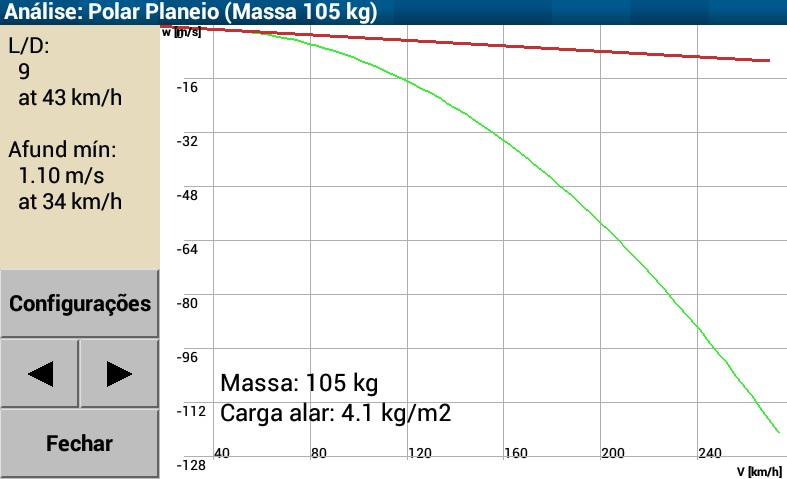
\includegraphics[angle=0,width=0.8\linewidth,keepaspectratio='true']{figures/analysis-glidepolar.png}
\end{center}

Dans cette page de dialogue, le bouton ``Paramètres'' ouvre la page ``Configuration vol'' et permet de régler en vol les paramètres `Ballast', `Moucherons', `QNH' et `Temp.\ max.'.

Quand le calculateur est connecté à un vario ``intelligent'' et supporté par \xc{} (ex~: Vega), la page Polaire de l'Analyse montre la moyenne de l'énergie totale du taux de chute en fonction de la vitesse horizontale.
Cette fonctionnalité permet aux pilotes de réaliser des vols de test en air stable et vent nul afin de mesurer la polaire réelle du planeur.
En comparant la polaire constructeur à celle mesurée, il est possible de contrôler / optimiser la vitesse de changement de position des volets, l'influence de l'étanchéité des ailerons et volets, etc.

Les données sont collectées uniquement en mode Transition et à un facteur de charge compris entre 0,9 et 1,1~g.
Les pilotes faisant des vols d'essais doivent donc voler dans un air stable et manœuvrer doucement les commandes en gardant les ailes horizontales.

\begin{center}
\includegraphics[angle=0,width=0.8\linewidth,keepaspectratio='true']{figures/shot-glidepolar.png}
\end{center}


\section{Notifications en vol}

Les notifications en vol, affichées comme des messages d'état, apparaissent dans les conditions suivantes~:
\begin{itemize}
\item Arrivée prévue en avance par rapport au temps donné d'un AAT.\@
\item Arrivée estimée après le coucher du soleil.
\item Changement important du vent (en intensité ou direction).
\item Passage au-dessus ou au-dessous du plan d'arrivée.
\end{itemize}
% JMW more detail here
